\chapter{Modellierung}
\section{Anforderungserhebung}
Wie in \autoref{theorie:referenzmodellierung} beschrieben, müssen Referenzmodelle einen subjektiven Empfehlungscharakter besitzen, damit sie akzeptiert und wiederverwendet werden. Dafür muss ein Abgleich mit den Anforderungen der Nutzenden geschehen. Um dies zu erreichen, wurden im Anhang transkribierte Interviews (Vgl. Anhang~\ref{chap:interview-philipp-22.03.2021}) \Todo{Hier RM-Interviews verlinken} durchgeführt. Daraus ergeben sich folgende Anforderungen an die zu konstruierenden Referenzmodelle:


\Todo{Anforderungstabelle}

\begin{figure}[H]
\centering
\spideroverview
%{P. Arnold}
{5}{3}{3}
%{R. Briegel}
{3}{3}{1}
%{P. Erbacher}
{2}{4}{5}
\caption{Ergebnisse der Interviews}
\label{abb:DimensionenUebersicht}
\end{figure}
\section{Echtzeitverarbeitung}

\begin{figure}[H]
\centering
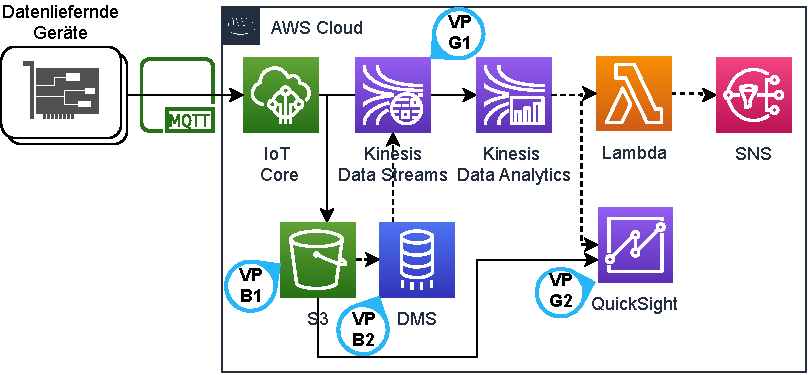
\includegraphics[width=\textwidth]{graphics/Echtzeit-RA-Overview.pdf}
\caption{Top Level View Referenzarchitektur}
\label{abb:TopLevelEchtzeitRA}
\end{figure}

\section{Datenbankseitige Verarbeitung}

\section{Einsatzszenarien der Referenzmodelle}